\section{Related work}

\subsection{Multi-objective path planning}

\begin{frame}{Graph based approach}{Multi-objective path planning}
\begin{itemize}
\item Discretization $ \rightarrow $ graph topology
\item Vector-based cost
\item Multi-objective A$ ^{*}$
\end{itemize}
Drawbacks
\begin{itemize}
\item information lose
\item discretization resolution
\end{itemize}
\end{frame}

\begin{frame}{Point-equivalence based approach}{Multi-objective path planning}
\begin{itemize}
\item Direction or waypoint 
\item Encode into solution
\item Evolutionary algorithm
\end{itemize}
Drawbacks
\begin{itemize}
\item obstacles $ \rightarrow $ discontinuity
\item giant search space
\end{itemize}
\end{frame}

\subsection{MOEA-D}

\begin{frame}{Decomposition method}{MOEA-D}
	Decompose a multi-objective optimization problem into subproblems
	\begin{itemize}
		\item Weighted sum approach
		\item Tchebycheff approach
		\item Boundary intersection approach
	\end{itemize}
\end{frame}

\begin{frame}{Weighted sum approach}{MOEA-D}
	\begin{columns}
		\column{0.5\textwidth}
		\begin{figure}
			\centering
			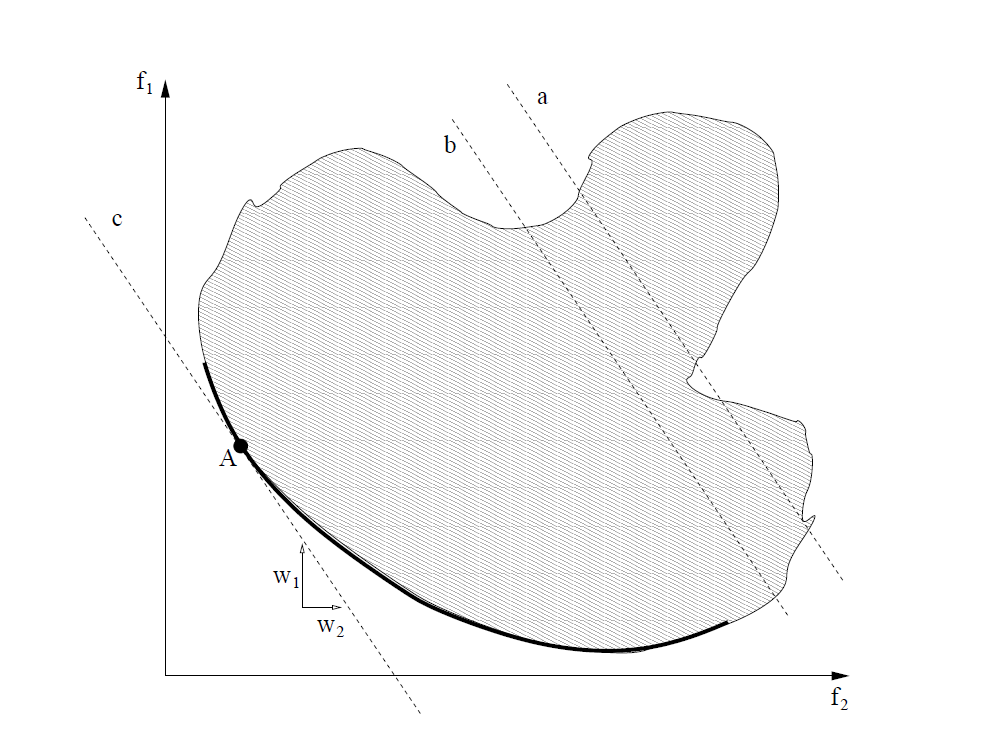
\includegraphics[width=\linewidth]{figure/weighted_sum}
			%\caption{}
			\label{fig:weighted_sum}
		\end{figure}
		\column{0.5\textwidth}
		\begin{minipage}{\textwidth}
			\begin{equation}
			\nonumber
			\arg\max_x \sum_{k=1}^{K} \lambda_{k} c_{k} (x)
			\end{equation}
			\begin{itemize}
				\item convex
			\end{itemize}
		\end{minipage}
	\end{columns}
\end{frame}

\begin{frame}{Tchebycheff approach}{MOEA-D}
	\begin{columns}
		\column{0.5\textwidth}
		\begin{figure}
			\centering
			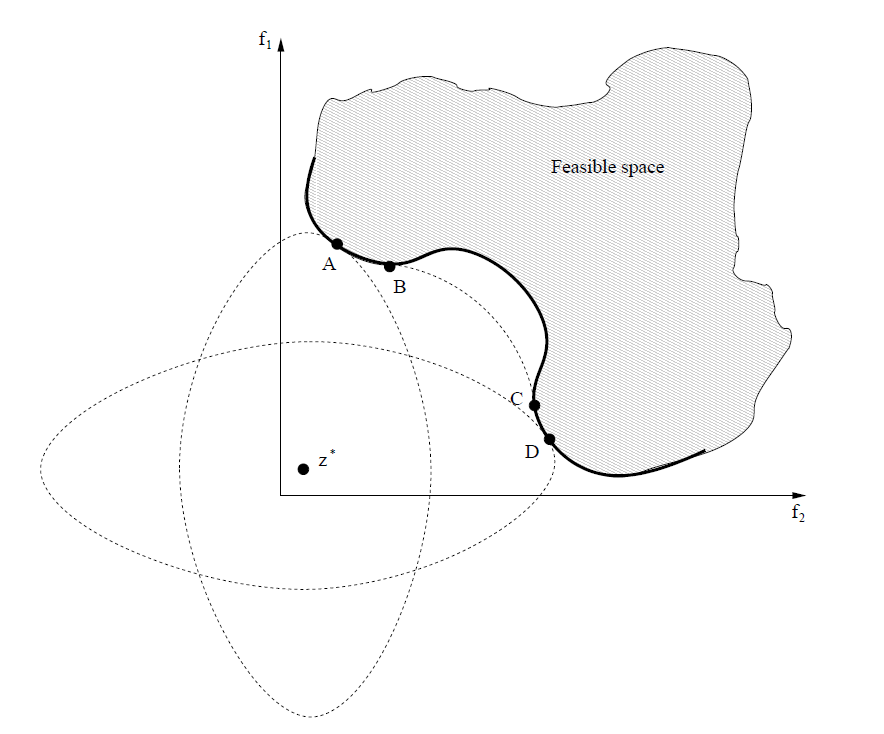
\includegraphics[width=\linewidth]{figure/tchebycheff}
			%\caption{}
			\label{fig:tchebycheff}
		\end{figure}
		\column{0.5\textwidth}
		\begin{minipage}{\textwidth}
            \begin{equation}
			\nonumber
			\arg\min_x \max_{1 \leq k \leq K}  \{ \lambda_{k} \mid c_{k}(x) - \bm{z}^{utop}_{k}  | \} 
			\end{equation}
			\begin{itemize}
				\item non-convex
			\end{itemize}
		\end{minipage}
	\end{columns}
\end{frame}

\begin{frame}{Boundary intersection approach}{MOEA-D}
	\begin{columns}
		\column{0.5\textwidth}
		\begin{figure}
			\centering
			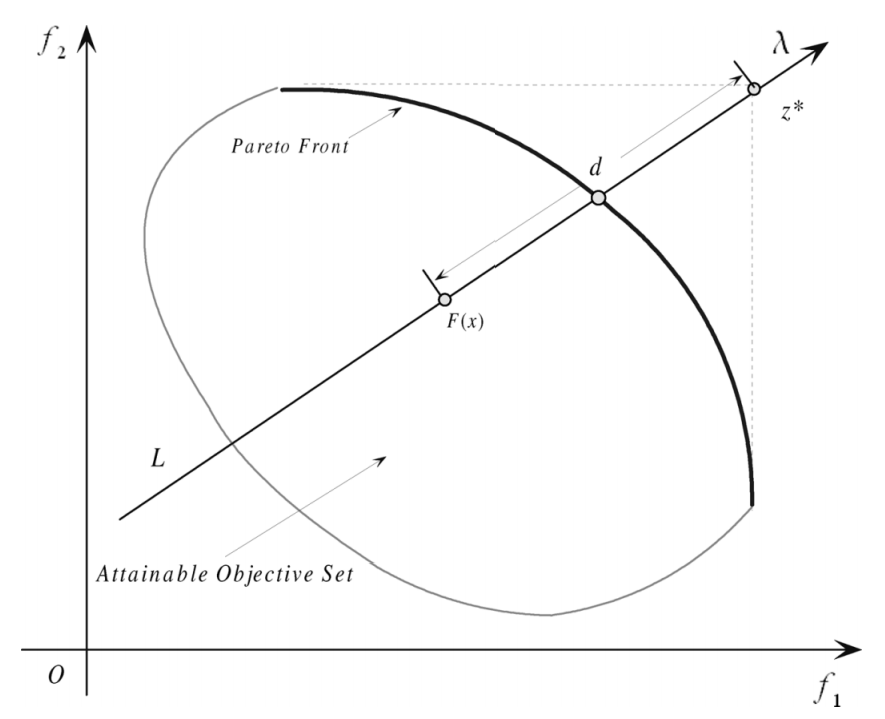
\includegraphics[width=\linewidth]{figure/boundary_intersection}
			%\caption{}
			\label{fig:boundary_intersection}
		\end{figure}
		\column{0.5\textwidth}
		\begin{minipage}{\textwidth}
			\begin{equation}
			\nonumber
			\arg \min_x \{ d \mid \bm{z}^{utop} - F(x) = d \bm{\lambda} \}
			\end{equation}
			\begin{itemize}
				\item better diversity
			\end{itemize}
		\end{minipage}
	\end{columns}
\end{frame}

\subsection{RRT$^{*}$}

\begin{frame}{RRT}{Sampling-based path planning}
	\begin{figure}
		\centering
		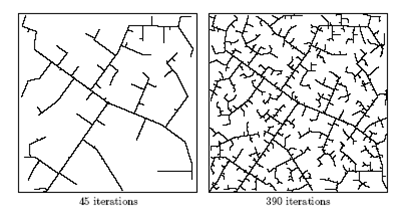
\includegraphics[width=.5\linewidth]{figure/RRT_graph1}
		%\caption{}
		\label{fig:rrt}
	\end{figure}
	\begin{figure}
		\centering
		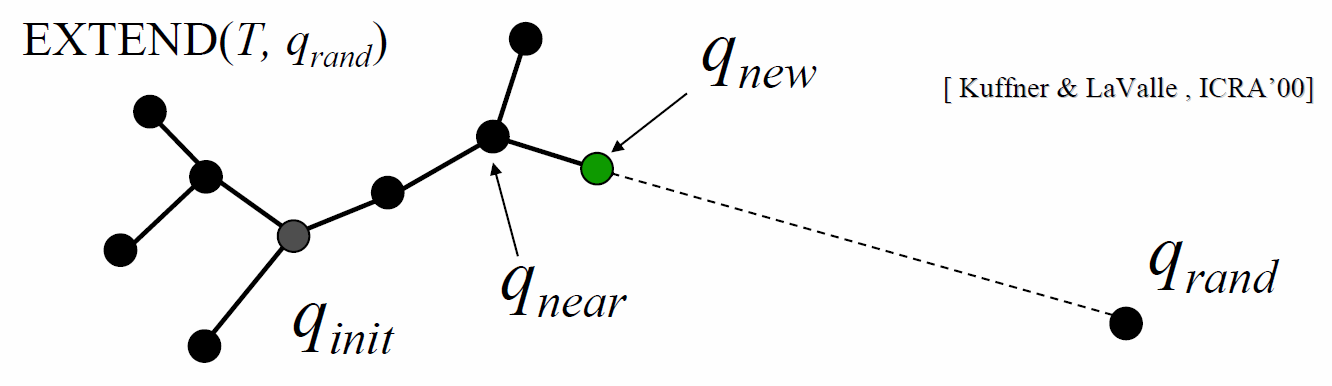
\includegraphics[width=.9\linewidth]{figure/rrt_extend}
		%\caption{}
		\label{fig:rrt_extend}
	\end{figure}
\end{frame}

\begin{frame}{RRT}{Sampling-based path planning}
	\begin{itemize}
	    \item simple (=efficient)
	    \item high degrees of freedom
		\item probabilistic complete 
		\item not asymptotic optimal
	\end{itemize}
\end{frame}


\begin{frame}{RRT$^{*}$}{Optimal sampling-based path planning}
{\Large \textbf{Sampling}}
\begin{columns}
	\column{0.33\textwidth}
	\begin{figure}
		\centering
		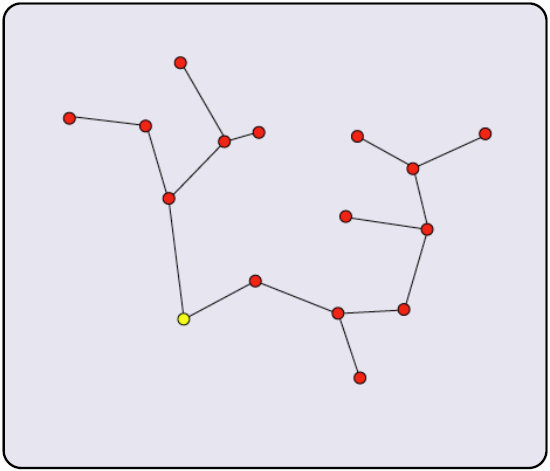
\includegraphics[width=\linewidth]{figure/RRTs00.png}
		%\caption{}
		\label{fig:rrts:00}
	\end{figure}
	\column{0.33\textwidth}
	\begin{figure}
		\centering
		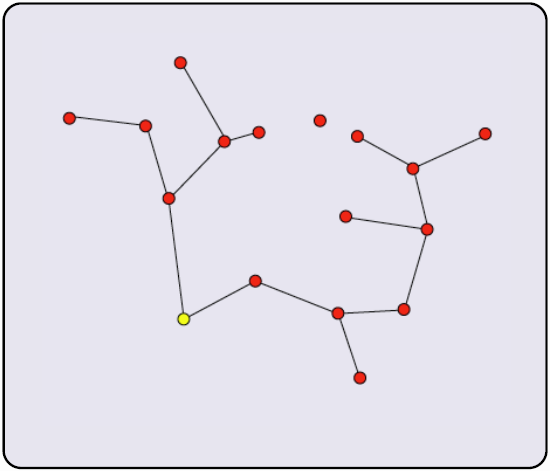
\includegraphics[width=\linewidth]{figure/RRTs01.png}
		%\caption{}
		\label{fig:rrts:01}
	\end{figure}
	\column{0.33\textwidth}
	\begin{figure}
		\centering
		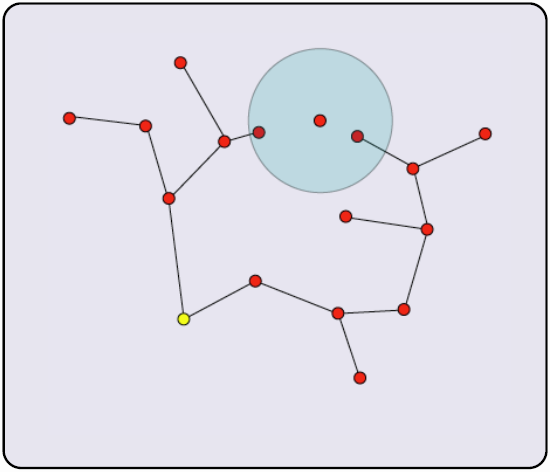
\includegraphics[width=\linewidth]{figure/RRTs02.png}
		%\caption{}
		\label{fig:rrts:02}
	\end{figure}
\end{columns}
\end{frame}

\begin{frame}{RRT$^{*}$}{Optimal sampling-based path planning}
{\Large \textbf{Adding}}
\begin{columns}
	\column{0.33\textwidth}
	\begin{figure}
		\centering
		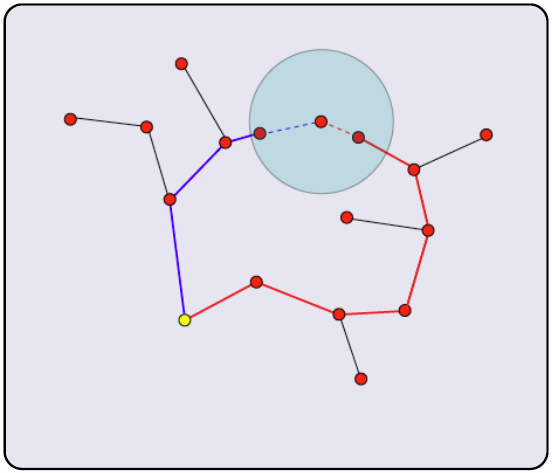
\includegraphics[width=\linewidth]{figure/RRTs03.png}
		%\caption{}
		\label{fig:rrts:03}
	\end{figure}
	\column{0.33\textwidth}
	\begin{figure}
		\centering
		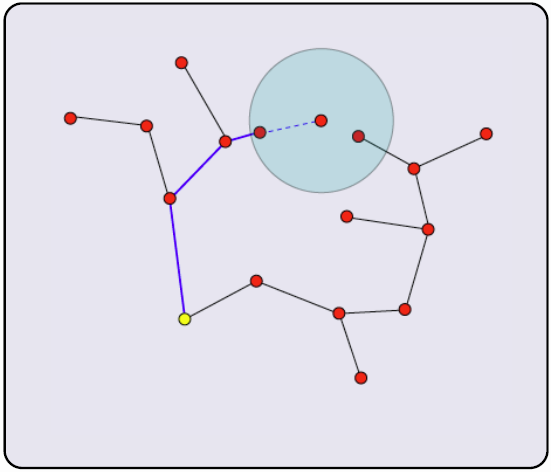
\includegraphics[width=\linewidth]{figure/RRTs04.png}
		%\caption{}
		\label{fig:rrts:04}
	\end{figure}
	\column{0.33\textwidth}
	\begin{figure}
		\centering
		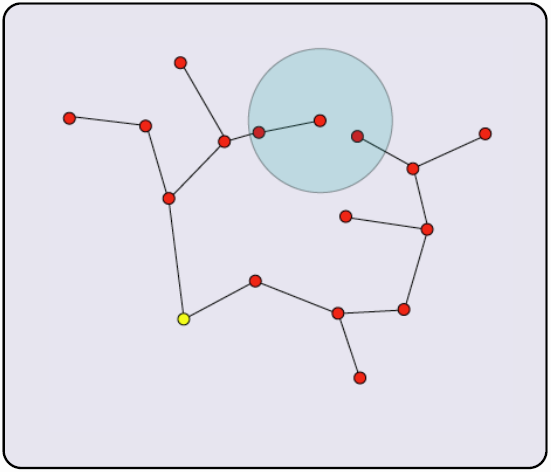
\includegraphics[width=\linewidth]{figure/RRTs05.png}
		%\caption{}
		\label{fig:rrts:05}
	\end{figure}
\end{columns}
\end{frame}

\begin{frame}{RRT$^{*}$}{Optimal sampling-based path planning}
{\Large \textbf{Rewiring}}
\begin{columns}
	\column{0.33\textwidth}
	\begin{figure}
		\centering
		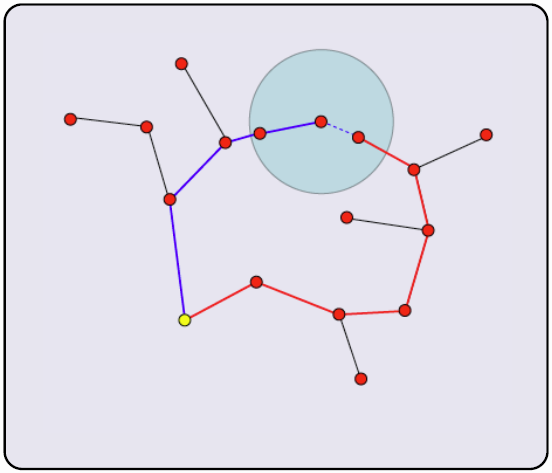
\includegraphics[width=\linewidth]{figure/RRTs06.png}
		%\caption{}
		\label{fig:rrts:06}
	\end{figure}
	\column{0.33\textwidth}
	\begin{figure}
		\centering
		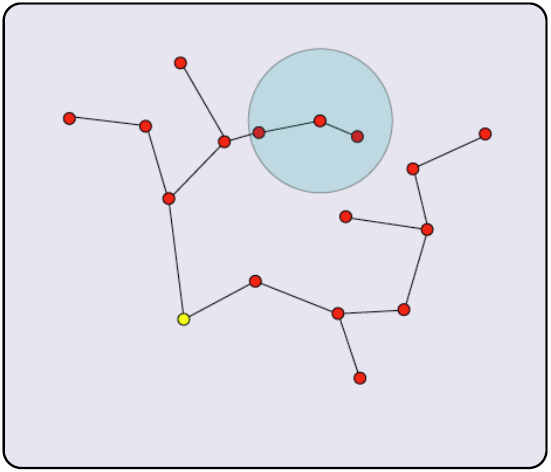
\includegraphics[width=\linewidth]{figure/RRTs07.png}
		%\caption{}
		\label{fig:rrts:07}
	\end{figure}
	\column{0.33\textwidth}
	\begin{figure}
		\centering
		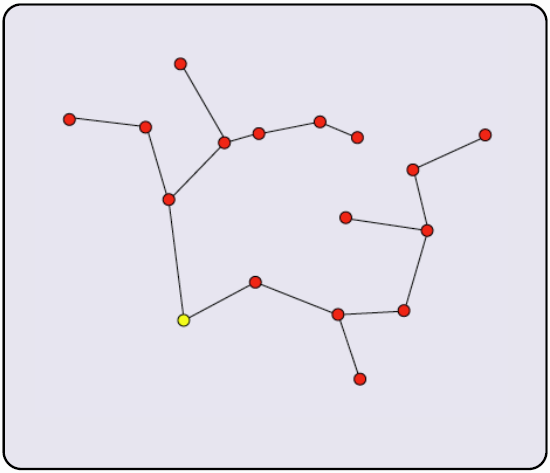
\includegraphics[width=\linewidth]{figure/RRTs08.png}
		%\caption{}
		\label{fig:rrts:08}
	\end{figure}
\end{columns}
\end{frame}

\begin{frame}{RRT vs RRT$^{*}$}{Optimal sampling-based path planning}
	\begin{figure}
		\centering
		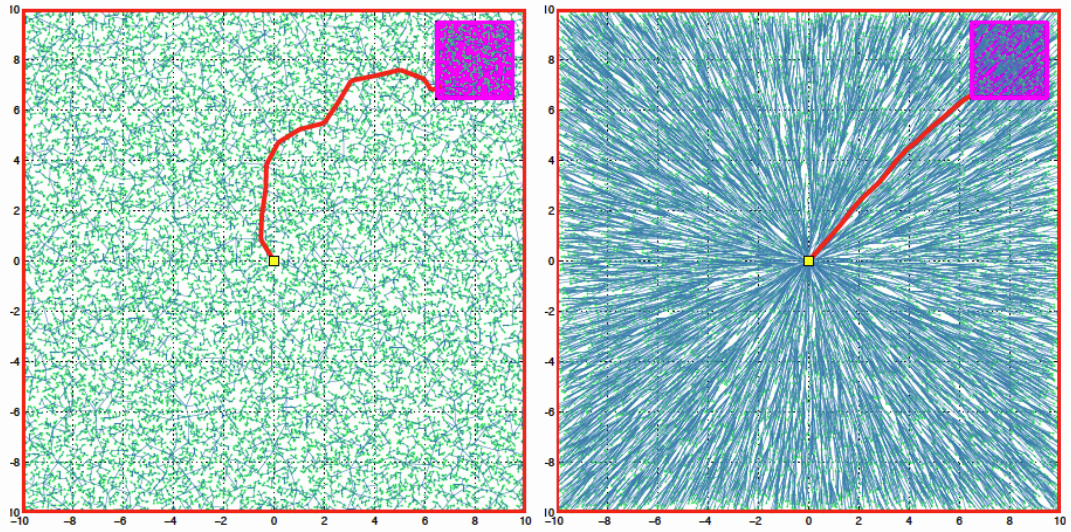
\includegraphics[width=.8\linewidth]{figure/RRT_RRTs.png}
		%\caption{}
		\label{fig:rrt:result}
	\end{figure}
\end{frame}
